\documentclass[10pt,a4paper]{article}


\usepackage[margin=22mm]{geometry}
\usepackage{amsmath,amsthm,amssymb,scrextend,graphicx,ifthen,hyperref}
\usepackage{fancyhdr}
\pagestyle{fancy}

\usepackage{todonotes}

\usepackage{color}

% ¤¤ Oversaettelse og tegnsaetning ¤¤ %
\usepackage[utf8]{inputenc}					% Input-indkodning af tegnsaet (UTF8)
\usepackage[british]{babel}					% Dokumentets sprog
\usepackage[T1]{fontenc}					% Output-indkodning af tegnsaet (T1)
\usepackage{hyperref}

\usepackage{csquotes}

% ¤¤ Matematik mm. ¤
\usepackage{amsmath,amssymb} 		% Avancerede matematik-udvidelser
\usepackage{mathtools}						% Andre matematik- og tegnudvidelser
\usepackage{setspace}
\usepackage[footnote,draft,danish,silent,nomargin]{fixme}
\usepackage[noend]{algpseudocode}

% ¤¤ Litteraturlisten ¤¤ %
\usepackage[backend=bibtex]{biblatex}

%Tikz%
\usepackage{tikz}
\usetikzlibrary{patterns}

\begin{document}
\lhead{SLIAL}
\chead{WS02: PageRanking}
\rhead{\today}

\fancyfoot[R] {\thepage}
\fancyfoot[C] {}
\fancyfoot[L] {} %{\small jaron@math.aau.dk}
\section*{Workshop - PageRank}
I denne Workshop betragter vi en person som surfer rundt på internettet. For at simplificere det en smule kigger vi kun på 5 mulige internetsider givet i mængden $W=\{w_1,w_2,w_3,w_4,w_5\}$. Vi antager, at personen via links på siderne går fra en af hjemmesiderne i mængden $W$ til en anden. Dette illustrerer vi ved de stokastiske variabler $W^{(t)}$. Udfaldet af $W^{(t)}$ er nummeret på den internetside personen er på på tidspunktet $t$. Lad nu sandsynlighederne for første udfald være
\begin{align}\label{eq:startfordeling}
	&P(W^{(0)}=1)=\frac{1}{2}, &&P(W^{(0)}=i)=\frac{1}{8}, \text{ hvor $i\in\{2,3,4,5\}$}.
\end{align}
Og sandsynlighederne for de resterende være
\begin{align*}
	&P(W^{(t+1)}=1|W^{(t)}=1)=0, &&P(W^{(t+1)}=i|W^{(t)}=1)=\frac{1}{4}\\
	&P(W^{(t+1)}=1|W^{(t)}=i)=\frac{1}{2}, &&P(W^{(t+1)}=i|W^{(t)}=j)=\frac{1}{8}
\end{align*}
for $i,j\in \{2,3,4,5\}$.
Dette er illustreret i Figur \ref{fig:Overgang}.
\begin{figure}[h!]
\centering
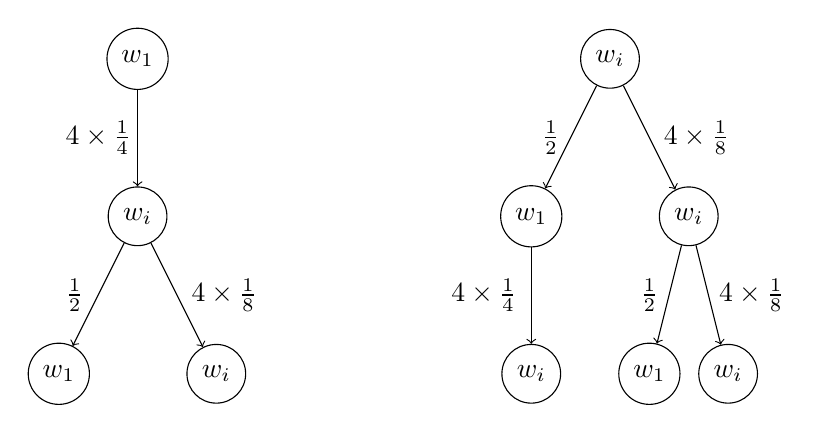
\begin{tikzpicture}
	\node[draw,circle] at (3, 0)   (W0-1) {$w_i$};
	\node[draw,circle] at (2, -2)   (W1-1-1) {$w_1$};
	\node[draw,circle] at (4, -2)   (W1-2-1) {$w_i$};
	\node[draw,circle] at (2, -4)   (W2-1-1) {$w_i$};
	\node[draw,circle] at (3.5, -4)   (W2-2-1) {$w_1$};
	\node[draw,circle] at (4.5, -4)   (W2-3-1) {$w_i$};

	 \draw[->] (W0-1) -- (W1-1-1);
	 \draw[->] (W0-1) -- (W1-2-1);
	 \draw[->] (W1-1-1) -- (W2-1-1);
	 \draw[->] (W1-2-1) -- (W2-2-1);
	 \draw[->] (W1-2-1) -- (W2-3-1);

	 \node[] at (2.25,-1)  {$\frac{1}{2}$};
	 \node[] at (4.1,-1)  {$4\times \frac{1}{8}$};
	 \node[] at (1.4,-3)  {$4\times \frac{1}{4}$};
	 \node[] at (3.5,-3)  {$\frac{1}{2}$};
	 \node[] at (4.8,-3)  {$4\times \frac{1}{8}$};


	\node[draw,circle] at (-3, 0)   (W0-0) {$w_1$};
	\node[draw,circle] at (-3, -2)   (W1-1-0) {$w_i$};
	\node[draw,circle] at (-4, -4)   (W2-1-0) {$w_1$};
	\node[draw,circle] at (-2, -4)   (W2-2-0) {$w_i$};

	 \draw[->] (W0-0) -- (W1-1-0);
	 \draw[->] (W1-1-0) -- (W2-1-0);
	 \draw[->] (W1-1-0) -- (W2-2-0);

	 \node[] at (-3.8,-3)  {$\frac{1}{2}$};
	 \node[] at (-1.9,-3)  {$4\times \frac{1}{8}$};
	 \node[] at (-3.5,-1)  {$4\times \frac{1}{4}$};
\end{tikzpicture}
\caption{Sandsynligheder. Til venstre ses, hvordan det vil se ud, hvis udfaldet i første eksperiment er $w_1$, hvilket sker med sandsynlighed $\frac{1}{2}$, og til højre ses hvordan det vil se ud, hvis udfaldet af første eksperiment er en af de andre $w_i$, $i=2,\dots,5$, hvilket sker med sandsynlighed $4\times \frac{1}{8}$ (dvs, sandsyndlighed $\frac{1}{8}$ for hver $i=2,\dots,5$).}
\label{fig:Overgang}
\end{figure}

Lad nu $X$ være en stokastisk variabel som t{\ae}ller hvor mange ganger internetside $1$ bes{\o}ges i tidsintervallet $t=0,1,2$.
Dvs
\[
X = \text{antallet af ganger\ } W^{(t)} = 1 \text{\ er opfyldt,\ } t=0,1,2.
\]

\subsection*{Delopgave 1}
\begin{enumerate}
\item Vi lader udfaldsrummet være $$S=\{w_iw_jw_k\mid i,j,k\in \{1,2,3,4,5\}\},$$ hvor hvert udfald svarer til de 3 internetsider bes{\o}gte i l{\o}bet af tidsintervalet $t=0,1,2$. Husk, at $X$ er en funktion fra $S$ til $\mathbb{R}$ og man kan derfor snakke om urbilledet af $y\in \mathbb{R}$, hvilket er givet ved $\{s\in S\mid X(s)=y \}$. Forklar, hvorfor dette urbillede svarer til en hændelse.
\item[\textbf{Svar}] Udfaldsrummet \textit{S} er alle de mulige udfald - deres sum er 1. Et udfald er givet ved $s$. Urbilledet af $y$ svarer til en hændelse da $S$ indeholder alle hændelser hvoraf $s$ er en enkelt hændelse.
\item For hvilke $y\in \mathbb{R}$ har vi et ikke-tomt urbillede? Og hvad er $p(X=y)$ for disse $y$?
\item[\textbf{Svar}] Vi har et ikke-tomt urbillede af $y$ hvis $X$ er opfyldt mellem 0 og 3 gange. Det er altså når $y \in \{0,1,2,3\}$ da det ikke vil være muligt at få $y=4$ da vi maks kan besøge side 1 i alt 3 gange og mindst 0 gange. 
\item[] \[p(X=0)=p(w_iw_iw_i)=\frac{1}{2} \cdot \frac{1}{2} \cdot \frac{1}{2}=\frac{1}{8}=0.125\]
		\[p(X=1)=p(w_1w_iw_i)+p(w_iw_1w_i)+p(w_iw_iw_1)=\frac{1}{2}\cdot 1 \cdot \frac{1}{2}+\frac{1}{2} \cdot \frac{1}{2} \cdot 1+\frac{1}{2}\cdot \frac{1}{2} \cdot \frac{1}{2}=\frac{5}{8}=0.625 \]  
		\[p(X=2)=p(w_1w_1w_i)+p(w_iw_1w_1)+p(w_1w_iw_1)=\frac{1}{2} \cdot 0 \cdot \frac{1}{2}+\frac{1}{2} \cdot \frac{1}{2} \cdot 0+\frac{1}{2} \cdot 1 \cdot \frac{1}{2}=\frac{2}{8}=0.25\]
		\[p(X=3)=p(w_1w_1w_1)=\frac{1}{2} \cdot 0 \cdot 0=0 \]
		Summen af sandsynligheden for disse fire udfald er 1.
\item Hvad er middelværdien og variansen for $X$?
\item[\textbf{Svar}] 
$
\text{Middelværdi: }\begin{aligned}[t] E(X)=\sum_{s\in S} p(s)X(s)&=0.125 \cdot 0+0.625 \cdot 1+0.25 \cdot 2=\mathbf{1.125}
\end{aligned} 
$
\\
$
\text{Varians: }\begin{aligned}[t] V(X) &= \sum_{s \in S} (X(s)-E(X))^2p(s) \\
&= (0-1.125)^2 \cdot 0.125 + (1-1.125)^2 \cdot 0.625+(2-1.125)^2 \cdot 0.25 = \mathbf{0.359375}
\end{aligned} 
$
\item Hvis $W^{(t)}$ i stedet havde fulgt en Bernoullifordeling for alle $t$ med sandsynlighed $\frac{3}{8}$ for at få $w_1$ (hvilket vi betegner som vores ``succes''), hvilken fordeling havde $X$ så fulgt og hvad havde middelværdien og variansen været? Sammenlign med det foregående eksempel.
\item[\textbf{Svar}]
\begin{align*}
	\begin{gathered}
		\text{Bernoulli trial}=b(k,n,p) \text{ where $k$=successes, $n$=independent trials, $p$=probability of success} \\
		b(k,n,p)=\text{C}(n,k)p^kq^{n-k} \\
		b\left(0;3;\frac{3}{8}\right)=\frac{3!}{0! \cdot (3-0)!} \cdot \frac{3}{8}^0 \cdot \left(1-\frac{3}{8}\right)^{3-0}=0.244140625 \\
		b\left(1;3;\frac{3}{8}\right)=\frac{3!}{1! \cdot (3-1)!} \cdot \frac{3}{8}^1 \cdot \left(1-\frac{3}{8}\right)^{3-1}=0.439453125 \\
		b\left(2;3;\frac{3}{8}\right)=\frac{3!}{2! \cdot (3-2)!} \cdot \frac{3}{8}^2 \cdot \left(1-\frac{3}{8}\right)^{3-2}=0.263671875 \\
		b\left(3;3;\frac{3}{8}\right)=\frac{3!}{3! \cdot (3-3)!} \cdot \frac{3}{8}^3 \cdot \left(1-\frac{3}{8}\right)^{3-3}=0.052734375 \\
	\end{gathered}
\end{align*}
	\begin{align*}
	\text{Middelværdi: }\begin{aligned}[t] E(X)=\sum_{s\in S} p(s)X(s)&=0.244140625 \cdot 0+0.439453125 \cdot 1+0.263671875 \cdot 2 + 0.052734375 \cdot 3=\mathbf{1.125}
	\end{aligned} 
\end{align*}
\begin{align*}
	\text{Varians: }\begin{aligned}[t] V(X) &= \sum_{s \in S} (X(s)-E(X))^2p(s) \\
	&= (0-1.125)^2 \cdot 0.244 + (1-1.125)^2 \cdot 0.439+(2-1.125)^2 \cdot 0.263+ (3-1.125)^2 \cdot 0.052 = \mathbf{0.703125}
	\end{aligned} 
\end{align*}
I forhold til den tidligere opgave så er middelværdien den samme, dog så er variansen forskellig.

\end{enumerate}

\begin{comment}
\[
\begin{gathered}
	\text{Bernoulli trial}=b(k,n,p) \text{ where $k$=successes, $n$=independent trials, $p$=probability of success} \\
	b(k,n,p)=\text{C}(n,k)p^kq^{n-k} \\
	b\left(0;2;\frac{3}{8}\right)=\frac{2!}{0! \cdot (2-0)!} \cdot \frac{3}{8}^0 \cdot \left(1-\frac{3}{8}\right)^{2-0}=0.390625 \\
	b\left(0;2;\frac{3}{8}\right)=\frac{2!}{1! \cdot (2-1)!} \cdot \frac{3}{8}^1 \cdot \left(1-\frac{3}{8}\right)^{2-1}=0.46875 \\
	b\left(0;2;\frac{3}{8}\right)=\frac{2!}{2! \cdot (2-2)!} \cdot \frac{3}{8}^2 \cdot \left(1-\frac{3}{8}\right)^{2-2}=0.140625 \\
\end{gathered}
\]
\end{comment}


Bemærk, at $W^{(t)}$ kan beskrives som en Markov-kæde med stokastisk matrix $P$ givet ved
\begin{align*}
	P=\begin{bmatrix}
		0 & \frac{1}{2} & \frac{1}{2} & \frac{1}{2} & \frac{1}{2}\\
		\frac{1}{4} & \frac{1}{8} & \frac{1}{8} & \frac{1}{8} & \frac{1}{8}\\
		\frac{1}{4} & \frac{1}{8} & \frac{1}{8} & \frac{1}{8} & \frac{1}{8}\\
		\frac{1}{4} & \frac{1}{8} & \frac{1}{8} & \frac{1}{8} & \frac{1}{8}\\
		\frac{1}{4} & \frac{1}{8} & \frac{1}{8} & \frac{1}{8} & \frac{1}{8}
	\end{bmatrix}
\end{align*}
I Delopgave $1$ betragtede vi kun $t=0,1,2$. Fra nu af begrænser vi os ikke til dette, men kan kigge på et vilkårligt $t\in \mathbb{N}$.
\subsection*{Delopgave 2}
\begin{enumerate}
	\item Hvad er sandsynligheden for at være i tilstand $w_1$ til tiden $t=5$, hvis vi bruger startfordelingen fra \eqref{eq:startfordeling} og den stokastiske matrix $P$?
	\item[\textbf{Svar}] \[ S=\begin{bmatrix}\frac{1}{2} & \frac{1}{8} & \frac{1} {8} & \frac{1} {8} & \frac{1} {8}\end{bmatrix}^T\]
		\[P^{(5)}=P^5P^{(0)}=\begin{bmatrix}
		0 & \frac{1}{2} & \frac{1}{2} & \frac{1}{2} & \frac{1}{2}\\
		\frac{1}{4} & \frac{1}{8} & \frac{1}{8} & \frac{1}{8} & \frac{1}{8}\\
		\frac{1}{4} & \frac{1}{8} & \frac{1}{8} & \frac{1}{8} & \frac{1}{8}\\
		\frac{1}{4} & \frac{1}{8} & \frac{1}{8} & \frac{1}{8} & \frac{1}{8}\\
		\frac{1}{4} & \frac{1}{8} & \frac{1}{8} & \frac{1}{8} & \frac{1}{8}
	\end{bmatrix}^5\begin{bmatrix}\frac{1}{2} & \frac{1}{8} & \frac{1} {8} & \frac{1} {8} & \frac{1} {8}\end{bmatrix}^T=\begin{bmatrix}
		\mathbf{0.328125} \\ 0.16796875 \\ 0.16796875 \\ 0.16796875 \\ 0.16796875
	\end{bmatrix}\]
	Det betyder altså at sandsynligheden for at være i tilstand $w_1$ (på internetside 1) ved tiden $t=5$ er $0.328125$.
	\item Har Markov-kæden en stationær fordeling? Hvis ja, bestem sådan en. 
	\item[\textbf{Svar}] Ja, Markov-kæden har en stationær fordeling da den kan beskrives som en stokastisk matrix. En stokastisk matrix er defineret ved en $N\times N$ matrix hvor alle værdier er ikke-negative. For at finde og bestemme den stationære fordeling skal vi løse ligningen $(P-I)x=0$. Så lad os gøre dette ved først at bestemme $P-I$:
	\[
	P-I=
	\begin{bmatrix}
		0 & \frac{1}{2} & \frac{1}{2} & \frac{1}{2} & \frac{1}{2}\\
		\frac{1}{4} & \frac{1}{8} & \frac{1}{8} & \frac{1}{8} & \frac{1}{8}\\
		\frac{1}{4} & \frac{1}{8} & \frac{1}{8} & \frac{1}{8} & \frac{1}{8}\\
		\frac{1}{4} & \frac{1}{8} & \frac{1}{8} & \frac{1}{8} & \frac{1}{8}\\
		\frac{1}{4} & \frac{1}{8} & \frac{1}{8} & \frac{1}{8} & \frac{1}{8}
	\end{bmatrix}-
	\begin{bmatrix}
		1 & 0 & 0 & 0 & 0 \\
		0 & 1 & 0 & 0 & 0 \\
		0 & 0 & 1 & 0 & 0 \\
		0 & 0 & 0 & 1 & 0 \\
		0 & 0 & 0 & 0 & 1
	\end{bmatrix}
	=
	\begin{bmatrix}
		-1 & \frac{1}{2} & \frac{1}{2} & \frac{1}{2} & \frac{1}{2} \\
		\frac{1}{4} & -\frac{7}{8} & \frac{1}{8} & \frac{1}{8} & \frac{1}{8} \\
		\frac{1}{4} & \frac{1}{8} & -\frac{7}{8} & \frac{1}{8} & \frac{1}{8} \\
		\frac{1}{4} & \frac{1}{8} & \frac{1}{8} & -\frac{7}{8} & \frac{1}{8} \\
		\frac{1}{4} & \frac{1}{8} & \frac{1}{8} & \frac{1}{8} & -\frac{7}{8} \\
	\end{bmatrix}
	\]
	Lad os nu beregne $(P-I)x=0$
	\[
	(P-I)x=0 \Longleftrightarrow 
	\begin{bmatrix}
		-1 & \frac{1}{2} & \frac{1}{2} & \frac{1}{2} & \frac{1}{2} & 0 \\
		\frac{1}{4} & -\frac{7}{8} & \frac{1}{8} & \frac{1}{8} & \frac{1}{8} & 0 \\
		\frac{1}{4} & \frac{1}{8} & -\frac{7}{8} & \frac{1}{8} & \frac{1}{8} & 0 \\
		\frac{1}{4} & \frac{1}{8} & \frac{1}{8} & -\frac{7}{8} & \frac{1}{8} & 0 \\
		\frac{1}{4} & \frac{1}{8} & \frac{1}{8} & \frac{1}{8} & -\frac{7}{8} & 0 \\
	\end{bmatrix}
	=
	\begin{bmatrix}
		1 & 0 & 0 & 0 & -2 & 0 \\
		0 & 1 & 0 & 0 & -1 & 0 \\
		0 & 0 & 1 & 0 & -1 & 0 \\
		0 & 0 & 0 & 1 & -1 & 0 \\
		0 & 0 & 0 & 0 & 0 & 0 \\
	\end{bmatrix} = \begin{matrix} x_1=2x_5 \\x_2=1x_5 \\x_3 =1x_5 \\ x_4=1x_5 \\x_5 \text{ is free} \end{matrix} \]
	\[ x_5= \begin{bmatrix}2 \\ 1 \\ 1 \\ 1 \\ 1 \end{bmatrix} \]
	\[q=\begin{bmatrix}2/6 \\ 1/6 \\ 1/6 \\ 1/6 \\ 1/6
\end{bmatrix}\]
	Markovkæden har altså en stationær fordeling som vi har bestemt til at være $q=\begin{bmatrix}2/6 & 1/6 & 1/6 & 1/6 & 1/6
\end{bmatrix}^T$. Den stationære fordeling betyder at der er større sandsynlighed for generelt at befinde sig på side 1 i forhold de andre 4 sider. 
\end{enumerate}

Bemærk at vi ovenfor antog, at vi kunne komme til alle andre internetsider via links uanset fra hvilken internetside vi kom fra. Det er måske fair nok i eksemplet ovenfor hvor vi kun betragter 5 sider, men ville nok ikke holde hvis vi betragtede flere sider. Bemærk, at vi stadig kan modellere det med en Markov-kæde, men at det blot vil betyde, at indgang $i,j$ i matricen for Markov-kæden er $0$, hvis der ikke er et link fra $w_j$ til $w_i$.

Vi kigger nu på et lidt større eksempel med $7$ hjemmesider, hvor der er links mellem siderne som illustreret på Figur \ref{fig:links}. Vi vil med dette som eksempel kigge nærmere på Google's PageRank algoritme.

\begin{figure}[h!]
\centering
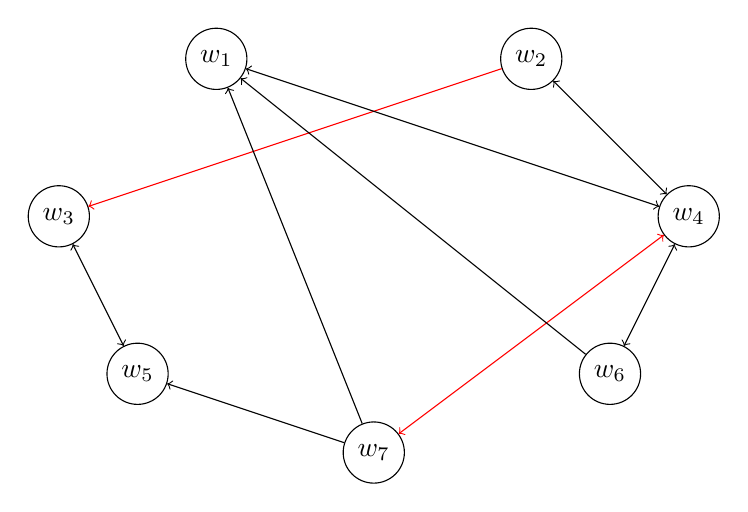
\begin{tikzpicture}[scale=1]
    % place nodes
    \node[draw,circle] at (-2, 2)   (w_1) {$w_1$};
    \node[draw,circle] at (2, 2)   (w_2) {$w_2$};
    \node[draw,circle] at (-4, 0)  (w_3) {$w_3$};
    \node[draw,circle] at (4, 0)  (w_4) {$w_4$};
    \node[draw,circle] at (-3, -2)  (w_5) {$w_5$};
    \node[draw,circle] at (3, -2)  (w_6) {$w_6$};
    \node[draw,circle] at (0, -3)  (w_7) {$w_7$};

    % draw edges
    \draw[red, ->] (w_2) -- (w_3);
	\draw[<->] (w_2) -- (w_4);
    \draw[<->] (w_4) -- (w_1);
	\draw[<->] (w_4) -- (w_6);
	\draw[<-] (w_5) -- (w_7);
	\draw[<->] (w_5) -- (w_3);
	\draw[->] (w_7) -- (w_1);
	\draw[red, <->] (w_7) -- (w_4);
	\draw[->] (w_6) -- (w_1);
\end{tikzpicture}
\caption{En pil fra en internetside til en anden betyder, at der er et link på den første til den anden side.}
\label{fig:links}
\end{figure}

I Google's PageRank algoritme betragter vi netop en person som surfer rundt på nettet. Vi bruger denne tænkte situation til at ``ranke'' internetsiderne. Den første tanke går på, at når surferen står på en side vil han vælge blandt de mulige links på siden med lige stor sandsynlighed. Derfor bliver den stokastiske matrix som illustrerer denne Markov kæde følgende (hvor både de røde og sorte pile tælles med)
\begin{align}\label{eq:Overgangsmatrix}
	P_1=\begin{bmatrix}
		0 & 0 & 0 & \frac{1}{4} & 0 & \frac{1}{2} & \frac{1}{3}\\
		0 & 0 & 0 & \frac{1}{4} & 0 & 0 & 0 \\
		0 & \frac{1}{2} & 0 & 0 & 1 & 0 & 0 \\
		1 & \frac{1}{2} & 0 & 0 & 0 & \frac{1}{2} & \frac{1}{3}\\
		0 & 0 & 1 & 0 & 0 & 0 & \frac{1}{3}\\
		0 & 0 & 0 & \frac{1}{4} & 0 & 0 & 0\\
		0 & 0 & 0 & \frac{1}{4} & 0 & 0 & 0
	\end{bmatrix}
\end{align}
Idéen i PageRank er mere eller mindre at finde sandsynligheden for at surferen er på en bestemt side efter ``tilstrækkelig mange'' klik. Det vi søger er altså en stationær fordeling.

\subsection*{Delopgave 3}
\begin{enumerate}
	\item Find stationær fordeling for Markov-kæden beskrevet ud fra den stokastiske matrix $P_1$.
	\item[\textbf{Svar}] \[P_1-I=\begin{bmatrix}
		0 & 0 & 0 & \frac{1}{4} & 0 & \frac{1}{2} & \frac{1}{3}\\
		0 & 0 & 0 & \frac{1}{4} & 0 & 0 & 0 \\
		0 & \frac{1}{2} & 0 & 0 & 1 & 0 & 0 \\
		1 & \frac{1}{2} & 0 & 0 & 0 & \frac{1}{2} & \frac{1}{3}\\
		0 & 0 & 1 & 0 & 0 & 0 & \frac{1}{3}\\
		0 & 0 & 0 & \frac{1}{4} & 0 & 0 & 0\\
		0 & 0 & 0 & \frac{1}{4} & 0 & 0 & 0
	\end{bmatrix}-\begin{bmatrix}
		1 & 0 & 0 & 0 & 0 & 0 & 0 \\
		0 & 1 & 0 & 0 & 0 & 0 & 0 \\
		0 & 0 & 1 & 0 & 0 & 0 & 0 \\
		0 & 0 & 0 & 1 & 0 & 0 & 0 \\
		0 & 0 & 0 & 0 & 1 & 0 & 0 \\
		0 & 0 & 0 & 0 & 0 & 1 & 0 \\
		0 & 0 & 0 & 0 & 0 & 0 & 1 \\
	\end{bmatrix}=\begin{bmatrix}
		-1 & 0 & 0 & \frac{1}{4} & 0 & \frac{1}{2} & \frac{1}{3}\\
		0 & -1 & 0 & \frac{1}{4} & 0 & 0 & 0 \\
		0 & \frac{1}{2} & -1 & 0 & 1 & 0 & 0 \\
		1 & \frac{1}{2} & 0 & -1 & 0 & \frac{1}{2} & \frac{1}{3}\\
		0 & 0 & 1 & 0 & -1 & 0 & \frac{1}{3}\\
		0 & 0 & 0 & \frac{1}{4} & 0 & -1 & 0\\
		0 & 0 & 0 & \frac{1}{4} & 0 & 0 & -1
	\end{bmatrix}\]
	\[
	(P_1-I)x=0 \Longleftrightarrow \begin{bmatrix}
		-1 & 0 & 0 & \frac{1}{4} & 0 & \frac{1}{2} & \frac{1}{3} & 0\\
		0 & -1 & 0 & \frac{1}{4} & 0 & 0 & 0 & 0 \\
		0 & \frac{1}{2} & -1 & 0 & 1 & 0 & 0 & 0 \\
		1 & \frac{1}{2} & 0 & -1 & 0 & \frac{1}{2} & \frac{1}{3} & 0\\
		0 & 0 & 1 & 0 & -1 & 0 & \frac{1}{3} & 0\\
		0 & 0 & 0 & \frac{1}{4} & 0 & -1 & 0 & 0\\
		0 & 0 & 0 & \frac{1}{4} & 0 & 0 & -1 & 0
	\end{bmatrix}
	=
	\begin{bmatrix}
		1 & 0 & 0 & 0 & 0 & 0 & 0 & 0 \\
		0 & 1 & 0 & 0 & 0 & 0 & 0 & 0 \\
		0 & 0 & 1 & 0 & -1 & 0 & 0 & 0 \\
		0 & 0 & 0 & 1 & 0 & 0 & 0 & 0 \\
		0 & 0 & 0 & 0 & 0 & 1 & 0 & 0 \\
		0 & 0 & 0 & 0 & 0 & 0 & 1 & 0 \\
		0 & 0 & 0 & 0 & 0 & 0 & 0 & 0 \\
	\end{bmatrix}
	\]
	Dette betyder at den stationære fordeling bliver $q$ hvor $x_5$ er free:
	\[w=\begin{bmatrix} 0\\0\\1\\0\\1\\0\\0\end{bmatrix},q=\begin{bmatrix} 0\\0\\0.5\\0\\0.5\\0\\0\end{bmatrix}\]
	\item Find stationær fordeling for Markov-kæden beskrevet ud fra Figur \ref{fig:links} hvis vi fjerner de røde pile. Derudover siger vi, at sandsynligheden for at gå fra en tilstand til den næste bliver fordelt ligeligt mellem de kanter der går ud fra tilstanden. (F.eks. går der to sorte pile væk fra $w_7$, hvorfor indgangene her bliver $\frac{1}{2}$).
	\item[\textbf{Svar}] Markov-kæden $P$ bliver dermed
	\[
	P=\begin{bmatrix}
		0 & 0 & 0 & \frac{1}{3} & 0 & \frac{1}{2} & \frac{1}{2} \\
		0 & 0 & 0 & \frac{1}{3} & 0 & 0 & 0 \\
		0 & 0 & 0 & 0 & 1 & 0 & 0 \\
		1 & 1 & 0 & 0 & 0 & \frac{1}{2} & 0 \\
		0 & 0 & 1 & 0 & 0 & 0 & \frac{1}{2} \\
		0 & 0 & 0 & \frac{1}{3} & 0 & 0 & 0 \\
		0 & 0 & 0 & 0 & 0 & 0 & 0
	\end{bmatrix}
	\]
	\[
	(P-I)x=0 \Longleftrightarrow \begin{bmatrix}
		1 & 0 & 0 & 0 & 0 & -\frac{3}{2} & 0 & 0 \\
		0 & 1 & 0 & 0 & 0 & -1 & 0 & 0 \\
		0 & 0 & 1 & 0 & -1 & 0 & 0 & 0 \\
		0 & 0 & 0 & 1 & 0 & -3 & 0 & 0 \\
		0 & 0 & 0 & 0 & 0 & 0 & 1 & 0 \\
		0 & 0 & 0 & 0 & 0 & 0 & 0 & 0 \\
		0 & 0 & 0 & 0 & 0 & 0 & 0 & 0
	\end{bmatrix}
	\]
	Efter at have lavet rækkeoperationer/row reduction så kommer vi frem til den overstående matrix. Deraf er løsningen:
		\[
		x=
		\begin{bmatrix}
			\frac{3}{2}x_6\\x_6\\x_5\\3x_6\\x_5\\x_6\\0 	
		\end{bmatrix}
		\]
		\text{Ved at vælge $x_5=1$ og $x_6$=1 får vi følgende}
		\[
		x=\begin{bmatrix}
			\frac{3}{2}\\1\\1\\3\\1\\1\\0
		\end{bmatrix}
		\]
		%\[
		%\frac{3}{2}x_6+x_6+x_5+3x_6+x_5+x_6=1 \Longleftrightarrow 6.5x_6+2x_5=1
		%\]
		\[
		%q=\begin{bmatrix}
		%\frac{\frac{3}{2}x_6 }{6.5x_6+2x_5}\\ \frac{x_6}{{6.5x_6+2x_5}} \\ \frac{x_5}{{6.5x_6+2x_5}} \\ \frac{3x_6}{{6.5x_6+2x_5}} \\ \frac{x_5}{{6.5x_6+2x_5}} \\ \frac{x_6}{{6.5x_6+2x_5}} \\ 0
		%\end{bmatrix}
		\]
		\[
		q=\begin{bmatrix}
			\frac{3}{2}/8.5 \\ 1/8.5 \\ 1/8.5 \\ 3/8.5 \\ 1/8.5 \\ 1/8.5 \\ 0
		\end{bmatrix}
		\]
		Vi har nu fundet den stationære fordeling hvor $x_5$ og $x_6$ er \textit{free variables}.
	
	\item Er der en entydig stationær fordeling i de to tilfælde? Kan I forklare hvorfor der er/ikke er?
	\item[\textbf{Svar}] For at der er en entydig stationær fordeling kræves det at den stokastiske matrix er \textbf{regular}, hvilket den er når alle elementer er positive og ikke nul i mindst en af $P^{(k)}$ potens (Theorem 18). Der findes ikke en entydig stationær fordeling i opgave 3.1 og 3.2 da ingen $P^k$ kun indeholder strengt positive indgange.
\end{enumerate}

Problemet med denne første tanke er, at vi ikke altid vil have en entydig stationær fordeling. For at sikre os, at vi altid opnår dette, tilføjer PageRank en sandsynlighed for at surferen starter et helt nyt sted (altså blot indtaster en ny internetadresse i stedet for at følge de links der er på siden).

Derfor benyttes i stedet den stokastiske matrix
\begin{align}\label{eq:PRmatrix}
	P=\alpha P_1+(1-\alpha)P_2
\end{align}
hvor $P_1$ er sandsynligheden via links (som vist i et eksempel i \eqref{eq:Overgangsmatrix}) og $P_2$ er en matrix hvor alle indgange er $1$ over antallet af tilstande/internetsider (i vores eksempel $\frac{1}{7}$). $\alpha$ er en variabel som kan justeres alt efter hvor sandsynligt, vi mener det er, at surferen følger links eller skifter til en ny side.

\subsection*{Delopgave 4}
\begin{enumerate}
	\item Hvorfor vil en Markov-kæde med stokastisk matrix $P$ som i \eqref{eq:PRmatrix} altid have en entydig stationær fordeling hvis $0<\alpha<1$?
	\item[\textbf{Svar}] \[
	P=\alpha \begin{bmatrix}
			0 & 0 & 0 & \frac{1}{4} & 0 & \frac{1}{2} & \frac{1}{3} \\
			0 & 0 &0 & \frac{1}{4} & 0 & 0 & 0 \\
			0 & \frac{1}{2} & 0 &0 & 1 & 0 & 0 \\
			1 & \frac{1}{2} & 0 &0 & 0 & \frac{1}{2} & \frac{1}{3} \\
			0 & 0 & 1 & 0 & 0 & 0 & \frac{1}{3} \\
			0 & 0 & 0 & \frac{1}{4} & 0 & 0 &0 \\
			0 & 0 & 0 & \frac{1}{4} & 0 & 0 &0
		\end{bmatrix}+(1-\alpha)\begin{bmatrix}
		\frac{1}{7} & \frac{1}{7} & \frac{1}{7} & \frac{1}{7} & \frac{1}{7} & \frac{1}{7} & \frac{1}{7} \\
		\frac{1}{7} & \frac{1}{7} & \frac{1}{7} & \frac{1}{7} & \frac{1}{7} & \frac{1}{7} & \frac{1}{7} \\
		\frac{1}{7} & \frac{1}{7} & \frac{1}{7} & \frac{1}{7} & \frac{1}{7} & \frac{1}{7} & \frac{1}{7} \\
		\frac{1}{7} & \frac{1}{7} & \frac{1}{7} & \frac{1}{7} & \frac{1}{7} & \frac{1}{7} & \frac{1}{7} \\
		\frac{1}{7} & \frac{1}{7} & \frac{1}{7} & \frac{1}{7} & \frac{1}{7} & \frac{1}{7} & \frac{1}{7} \\
		\frac{1}{7} & \frac{1}{7} & \frac{1}{7} & \frac{1}{7} & \frac{1}{7} & \frac{1}{7} & \frac{1}{7} \\
		\frac{1}{7} & \frac{1}{7} & \frac{1}{7} & \frac{1}{7} & \frac{1}{7} & \frac{1}{7} & \frac{1}{7} \\
	\end{bmatrix}
	\]
	Når $0<\alpha<1$ så vil alle indgange/entries være strengt/strictly positive og dermed er $P$ en regulær stokastisk matrix. $P^1$ indeholder nemlig kun positive tal hvilket ved definition i Theorem 18 derfor har en entydig stationær fordeling.
	\item Forklar hvad et lille/stort $\alpha$ betyder for vores vurdering af surferens adfærd.
	\item[\textbf{Svar}] 
		\begin{enumerate}
			\item[] Et lille $\alpha$ vil betyde at der er stor sandsynlighed for at brugeren blot indtaster en ny internetadresse i stedet for at følge links på siden. 
			\item[] Et stort $\alpha$ må så betyde at der er stor sandsynlighed for at brugeren følger links på siden.
		\end{enumerate}
	\item Beregn den entydige stationære fordeling for de to eksempler i Delopgave 3 hvis vi sætter $\alpha=0.85$, som typisk er blevet brugt i literaturen. Ud fra resultaterne, hvordan vil I så ``ranke'' internetsiderne i de to eksempler?
	\item[\textbf{Svar}]
	Ved at reducere $P=\alpha P_1+(1-\alpha)P_2$ til reduced row-echelon form (ved brug af MATLAB) får vi følgende værdier.
	\begin{align*}
		\begin{bmatrix}
			1 & 0 & 0 & 0 & 0 & 0 & -1.7083 & 0 \\
			0 & 1 & 0 & 0 & 0 & 0 & -1 & 0 \\
			0 & 0 & 1 & 0 & 0 & 0 & -4.8769 & 0 \\
			0 & 0 & 0 & 1 & 0 & 0 & -2.9570 & 0 \\
			0 & 0 & 0 & 0 & 1 & 0 & -4.8003 & 0 \\
			0 & 0 & 0 & 0 & 0 & 1 & -1 & 0 \\
			0 & 0 & 0 & 0 & 0 & 0 & 0 & 0
		\end{bmatrix}
	\end{align*}
	Deraf kan vi nu finde en simpel basis for løsningen:
	\begin{align*}
		x_7 = \begin{bmatrix}
			1.7083 \\ 1 \\ 4.8769 \\ 2.9570 \\ 4.8003 \\ 1 \\ 1
		\end{bmatrix}
	\end{align*}
	Ved at dividere hver indgang med summen af alle indgange får vi nu sandsynlighedsvektoren $\mathbf{q}$.
	 \[\mathbf{q}=
	 \begin{bmatrix}
		 1.7083/17.3425 \\ 1.000/17.3425 \\ 4.8796/17.3425 \\ 2.9570/17.3425 \\ 4.8003/17.3425 \\ 1/17.3425 \\ 1/17.3425
	 \end{bmatrix}
	 =
	 \begin{bmatrix}
		0.0985048\\0.05766135\\0.28120974\\0.17050718\\0.27679424\\0.05766135\\0.05766135
	\end{bmatrix}\]
	Denne entydige stationære fordeling $\mathbf{q}$ (steady-state vector) fortæller os at den mest vigtige internetside er nr. 3 efterfulgt af henholdsvis 5, 4, 1 og 2, 6, 7. Derfor vil jeg "ranke" internetsiderne i netop denne rækkefølge hvor side 3 er mest vigtig og 2,6,7 er mindst vigtige.\\
	Hvis vi kigger på det andet eksempel så får vi
	\begin{align}
		x_7=\begin{bmatrix}
			7.1058 \\ 4.6883 \\ 7.9685 \\ 13.0176 \\ 8.1982 \\ 4.6883 \\ 1
		\end{bmatrix}
	\end{align}
	Og så dividere vi med summen af alle indgange og får sandsynlighedsvektoren $\mathbf{q}$.
	\begin{align}
		\mathbf{q}=\begin{bmatrix}
			7.1058/46.6667 \\ 4.6883/46.6667 \\ 7.9685/46.6667 \\ 13.0176/46.6667 \\ 8.1982/46.6667 \\ 4.6883/46.6667 \\ 1/46.6667
		\end{bmatrix}=\begin{bmatrix}
			0.15 \\ 0.10 \\ 0.17 \\ 0.28 \\ 0.18 \\ 0.10 \\ 0.02
		\end{bmatrix}
	\end{align}
	Jeg vil ranke siderne fra mest vigtig til mindst vigtig på følgende måde: $w_4,w_5,w_6,w_1,w_2,w_6,w_7$.

\end{enumerate}
\end{document}
